\section{Background}\label{sec:background}

TODO introduction
\subsection{Spark}
Spark is the probably most widely used and industry accepted cluster computing model.
It improves over former computing models, e.g. MapReduce~\cite{mapreduce}, Hadoop~\cite{Hadoop} or Haloop~\cite{haloop},
by allowing to cache results in memory between multiple queries, using so-called resilient
distributed datasets~\cite{rdd}; often abbreviated to RDD. % TODO sources for hadoop and haloop

\subsubsection{Spark architecture}
Spark allows the user to run his program on a single machine or on hundreds of machines organized in a cluster.
In this section, we explain the architecture that allows this flexibility.
\Cref{fig:spark-cluster} shows a schematic Spark cluster setup.

\begin{figure}
    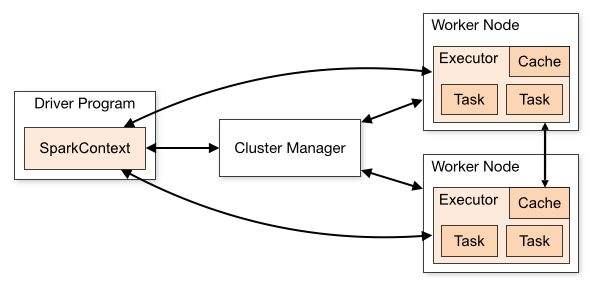
\includegraphics[width=\textwidth]{figures/spark-cluster.png}
    \caption{
      Schematics of a Spark cluster with two workers, each of them with one exectuor and two threads per executor.
      Source: Apache Spark Documentation~\footnote{https://spark.apache.org/docs/latest/cluster-overview.html}
    }
\end{figure}

In Spark, each physical machine is called a \textit{worker}.
On each worker, Spark starts one or multiple Spark processes in their own JVM instance; each of them is called \textit{executor}.
Nowadays, many Spark deployments use a single executor per worker\footnote{This is the setup Databricks uses; Databricks is the leading
maintainer of the Spark platform and offers professional deployment to many customers.}
Each executor runs multiple threads (often one per core on its worker) to execute multiple tasks in parallel.
In total, a Spark cluster can run \textit{\# workers} $\times$ \textit{\# executors per worker} $\times$ \textit{\# threads per executor} tasks
in parallel.

Spark uses two kind of processes to execute an application: a \textit{driver program} and multiple \textit{executors}.
When started, the driver program aquires resources from the \texit{cluster manager} to start its executors.
These executors stay alive during the whole Spark application.
Then, the driver program then continues executing the Spark application.
When it encounters parallelizable tasks, it schedules them on the available executors.

All tasks scheduled on the same executor share a cache for in memory data structures like \textit{Broadcast variables} or persisted RDD
partitions.
This is important in the context of this thesis because it means that we cache the input graph once per executor;
which in many Spark deployments is once per worker or physical machine.
This would not be possible if different tasks in the same JVM would not share the same cache.

Spark allows the user to choose its own cluster manager to manage resources in the cluster.
It comes with good integration for Hadoop YARN~\cite{yarn}, Apache Mesos~\cite{mesos} and Kubernetes~\cite{kubernetes}, as well as,
an standalone mode where it provides its own cluster manager functionality.
Finally, one can run Spark in \textit{local mode} on a single machine using multiple processor cores for worker threads.
In local mode, the driver program and a single executor with as many threads as cores to use share a single JVM.
For our experiments, we run Spark purely in local mode.

\subsubsection{Resilient distributed datasets}
RDD's form the core of Spark.
However, for this thesis it is not necessary to understand them in great detail.
In the next paragraph, we give a short introduction into the relevant aspects of RDD's.
For the interested reader, a more in depth description is given in the original paper~\cite{RDD}.

Resilient distributed datasets describe a distributed collection of data items of a single type.
In contrast, to other distributed share memory solutions, RDD's do not use fine-grained
operations to manipulate single data items but coarse grained operation that are applied
to all data items, e.g. \textit{map} to apply a function to each data item.
These operations are called transformations.
An RDD is built starting from a persistent data source and multiple transformation to
apply to this datasource.
One can store the transformations applied to the input data source as in directed acyclic graph, the so called \textit{lineage graph}.
This graph fully describes the dataset without materializing it because the transformations are deterministic.
Hence, the dataset can be computed and recomputed on demand, e.g. when the user asks for the count
of all items in the set.
Operations which require that the data in the RDD is actually computed are called \textit{actions}.

RDD's are distributed by organizing their data items into partitions.
The partitioning can be chosen by the user or the Spark query optimizer such that it allows to run transformations on all partitions
in parallel.
For example, one might chose a round robin paritioning to generate splits of equal size when reading data items from disk or one
groups items by hashing a specific key to support parallelizable aggregation on that key per partition.

Describing datasets as RDD's comes with two main benefits.
First, it is resilient because if the dataset of some partitons of it get lost, it is possible to recompute them from persistent storage
using lineage graph information.
Second, it allows Spark to compute RDD's in parallel.

Spark can parallelize the computation of RDD in two ways.
First, by data-parallelism due to the fact that different partitions of a RDD can
be computed in independently from each other.
Second, by task parallelism due to the fact that some parts of the DAG can be computed without dependence of the others.
Indeed, it is possible to compute all parts of an RDD in parallel which are not related in a topological sort of the graph.

%We show the lineage graph of a triangle count query in Spark in \cref{fig:lineage-triangle}.
%The triangle query is given by the datalog rule
%$COUNT(triangle(A, B, C)) \leftarrow R(A, B), S(B, C), T(A, C), A < B < C $.
%We explain the figure from top to bottom.
%Each vertice in the graph represents a transformation.
%The sources of the DAG are persistent data sources.
%In this case, the edge relationship of the graph given by a CSV file.
%All source vertices are filtered to fulfill $A < B < C$, while being written from disk.
%The two left most source vertices are the lineage parents of the join between \textit{R}
%and \textit{S} via \textit{B}.
%The result of this join and the last relationship \textit{T} are input to the second
%join.
%Finally, we see the count action which aggregates the result of the last join.




%We give examples for both kind of parallelism in the triangle count query
%(\cref{fig:lineage-triangle}).
%Lets assume that the CSV file is partitioned in 10 equal parts and each part is read
%by one out of 10 workers.
%Then the resulting RDD has 10 partitions.
%The following filter can be applied to all 10 partitions in parallel.
%This computation is also task parallel because all three filters can be applied to the
%input set directly after reading it from disk.

%If we go one step further into the example of the triangle query and look at the first
%join, we see limitations to Spark's parallelism.
%Let's assume that we want to use a Hashjoin implementation.
%In this case, we have to build a hash table of either side of the join.
%Hence, the computation of the join needs to wait until this hash table has been build.
%This is clearly not task parallel and it's also not data parallel on the build site
%because we need the data from all partitions to construct a full hash table.
%The result is that we see an exchange operator in the DAG of \cref{fig:triangle-lineage}.
%This operator allows to reorganize the partitions of a RDD.
%In the case of a hash join, it would reorganize items from all partitions into a hash
%table and make copies of this hash table available to the tasks that compute the
%partitions of the join.

%In the last paragraphs, we covered that Spark uses data parallelism arising from the partitioning of the RDD's
%and task parallelism arising from the lineage-graph representation of the RDD's.
%Synchronization happens via exchange operators which allow to reorganize the paritioning of the RDD's.
%In the following, we explain how Spark exploits parallelism in its execution model.

% TODO turn reasoning around? Stages to tasks?
%Spark uses a scheduler to assign \textit{tasks} to \textit{slots}.
%\textit{Tasks} are the smallest unit of work in Spark.
%They are created by dividing the RDD lineage graph into pipelinable \textit{stages}.
%Normally, a stage consists out of all transformations between two exchange operators.
%Each stage consists out of as many tasks as it has partitions.

%The stages of the triangle query are shown in \cref{fig:triangle-lineage}.
%We have four stages.
%Two to build the hash table for our hash join which start with reading the CSV from disk and end with the exchange operator before
%the join.
%The longest stage also reads the CSV from disk, includes the two streaming sites of the hash joins and finally aggregates all
%results per partition for the count.
%It ends with an exchange to aggregate the counts of all partitions; this aggregation is the last out of for \textit{stages}.
%
%These four stages lead to 31 tasks if we assume that each stage starts with reading the CSV into 10 partitions.
%This is because the first 3 stages have 10 tasks each and the last stage accumulating all counts after the last task is only as single
%task of summing up all partitions of its parent.


\subsection{Broadcast variables}
From the programmer point of view, \textit{broadcast variables} are normal readonly variables.
They are initialized once by the driver program and should not be changed after initialization.
Every serializable type can be used for a broadcast variable.
After intitialization they can be accessed by every task.
When they are not cached the task aquires the value of the variable from the driver program or other workers, deserializes it and
adds it to the cache shared by all tasks on the machine.
Spark guarantees that the each broadcast variable is sent only once to each executor and allows it to be spilled to disk if its not
possible to keep the whole value in memory.
Furthermore, `Spark attempts to distribute broadcast variables using efficient broadcast algorithms to reduce communication
costs'~\cite{rdd-programming-guide}; currently Spark uses a BitTorrent-like communication protocol\footnote{See Spark sources: \texttt{org
.apache.spark.broadcast.TorrentBroadcast}}.
% TODO cite https://spark.apache.org/docs/2.2.0/rdd-programming-guide.html


% Shuffles in Spark...
However, although Spark implements most operations in memory, shuffles are an exception which still writes and reads
the whole intermediary dataset to and from disk.
Consequently, shuffling remains to be a highly expensive operation which is the bottleneck of many workflows.
Still, Spark provides the user with a general distributed data processing model with strong fault- and struggler tolerance
on commodity, shared-nothing clusters.

\subsubsection{Catalyst}
Catalyst~\cite{catalyst} is Spark's query optimizer.
From a given query, e.g. an SQL query or one constructed using the DataFrame API, it constructs
in multiple stages an executable \textit{physical plan}.
\begin{figure}
    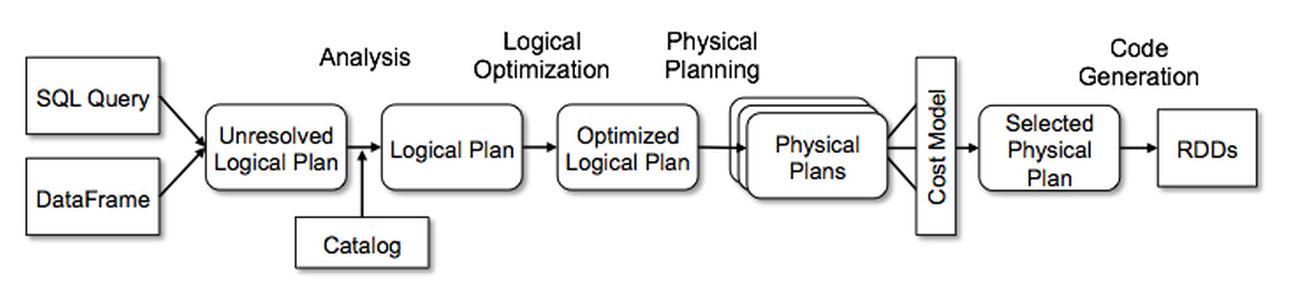
\includegraphics{figures/catalyst-stages.png}
    \caption{Input and stages of the Catalyst optimizer.}
    \label{fig:catalyst-stages}
\end{figure}
Its inputs and stages are shown in~\cref{fig:catalyst-stages}.
Below we explain these in order.

The input of Catalyst is a query in the form of a DataFrame or SQL string.
From the optimizer builds a \textit{unresolved logical plan}.
This plan can include unresolved attributes, e.g. attribute names which are not matched to a specific
data source yet or which have no known type.
To resolve this attributes Catalyst uses a \textit{Catalog} of possible bindings which describes the
available data sources.
This phase is referred to as \textit{Analysis} and results in a \textit{logical plan}.

The \textit{logical plan} represents \textit{what} should be done for the query but not exactly \textit{how},
e.g. it might contain a Join operator but not a Sort-merge join.
The logical optimization phase applies batches of rewriting rules until a fixpoint is reached.
A simple example of a logical optimization would be rewriting $2 + 2$ into $4$.

From the \textit{optimized logical plan} the optimizer generates one or multiple \textit{physical plans} by
applying so called \textit{Strategies}.
They translate a logical operator in one or multiple physical operators.
\textit{Strategies} are also allowed to return multiple physical plans for a single \textit{logical plan}.
In this case, the optimizer selects the best one according to a \textit{cost model}.

During the \textit{code generation} phase, Catalyst compiles Java byte code for some of the \textit{physical
operators}.
This code executes often magnitudes faster than interpreted versions~\cite{catalyst} of the same operator because
it can be specialized towards this particular query, e.g. if a join operates only on integers, code
generation can prune all code paths dealing with strings.
% TODO cite paper or website?
Indeed, the code generation phase is part of another Spark project called \textit{Tungsten}~\cite{tungsten}.
In this thesis, we do not build any code generated physical operators.
Hence, we do not treat this topic in depth.
It is enough to know that all freshly generated Java code is wrapped into physical operators of the type \textit{WholeStageCodeGen}
which allows seamless integration with interpreted operators.

Finally, Catalyst arrives at an optimized physical plan which implements the query.
The execution of this plan is called
\textit{structured query execution}~\cite{spark-internals-structured-query-execution}.
% TODO cite https://jaceklaskowski.gitbooks.io/mastering-spark-sql/spark-sql-QueryExecution.html
It translates the plan into RDD operations implemented by Spark core.
Hence, the result of Catalysts query compilation is an RDD representing the query.
One should note that \textit{structured query execution} does not actually execute the query: the result is an RDD which is a none
materialized representation of the operations necessary to generate the
result.
In this thesis, we are not concerned with the internals of RDD's.
We do not need to introduce any new RDD operations or even touch Spark's core functionality.
Thanks to the extensibility of Catalyst, we can integrate worst-case optimal joins by adding one \textit{logical operator}, multiple
\textit{physical operators} and a \textit{Strategy} to translate the \textit{logical operator} in
its physical implementation.

\subsection{Worst-case optimal join algorithm}
The development of worst-case optimal joins started in 2008 with the discovery that the output size of a relational query is bound by the fractional edge number of its underlying hypergraph~\cite{agm}.
In 2012, Ngo, Porat, Re and Rudra published a join algorithm matching this bound~\cite{nprr}.
In the same year, Veldhuizen proved that the algorithm ``Leapfrog Triejoin'' used in LogicBlox, a database system developed by his company, is also worst-case optimal with regards to the
fractional edge number bound.
Both alorithms have been shown to be instances `Generic Join' in 2013 Ngo et al.~\cite{skew-strikes-back}.
Leapfrog Triejoin is the only worst-case join algorithm that has been implemented and benchmarked numerous times in widely different settings, e.g. Oxford course work, published research and a commercial database system~\cite{leapfrog,andreas,olddog,myria,ammar2018distributed,leapfrog-triejoin-schroeder}.

\subsubsection{LeapfrogTriejoin}
% TODO LFTJ chapter

\subsection{Distributed worst-case optimal join in Myria}
In 2014, a Leapfrog Triejoin variant, dubbed ``Tributary Join'', was used as a distributed join algorithm on a shared-nothing architecture called ``Myria''~\cite{myria-detailed}.
They use Tributary Join as a local, serial worst-case optimal join algorithm, combined with the Hypercube shuffle algorithm to partition the data between their machines~\cite{hypercube}.
% TODO sort out hypercube and shares usage
However, it is not obvious how well Hypercube shuffles scales because it replicates many of its input tuples~\cite{myria-detailed}.
The combination of Hypercube shuffles and Tributary Join in Myria does not scale well (speedup of 8 on 64 workers compared to the time it takes on 2 nodes) which, although unlikely to be optimal, is not investigated in great detail; we therefore, explain Hypercube shuffles in detail and show that they tend to replicate all data to all nodes for bigger graph patterns~\cref{ssec:hypercube-shuffle}.
Their approach is directly applicable to Spark.
% TODO add Graphflow paper: variable ordering studied, combination of bin + wcoj in plans, query planning first known approach, parallel
% execution?
% TODO check emptyheaded, it uses WCOJ's

\subsubsection{Shares}
% TODO rename HC Shares
We first explain how the Hypercube shuffle algorithm, \texttt{HC}, partitions data.
After, we provide an analysis of its scaling with regards to graph patterns with an increasing number of vertices.

\texttt{HC} partitions the input relationships for a multi-way join over \textit{w} worker nodes, such that, all tuples, which could be joined, end up on the same worker in a single shuffle round.
Hence, it allows running any multi-way join algorithm locally after one shuffle round.
The output of the join is the union of all local results.
\texttt{HC} realizes this partitioning by logical organizing all workers in a hypercube with one dimension per join variable; we call the number of variables \textit{A} and use $a_i$ to reference a single variable.
Each dimension has a size $p_i$, the $p_i$'s have to be chosen such that the constraint $w \ge \prod_{i}p_i$ is satisfied.  % TODO choosing problem
In other words, each worker can be addressed by its coordinate in the hypercube of the form $\{1..p_1\} \times ... \times \{1..p_A\}$.

With this topology in mind, it is straightforward to find a partitioning for all tuples from all relationships such that tuples that could join are sent to the same node.
We choose a hash function $h_i$ for each join variable which maps its values in the range of \{1..$p_i$\}.
Then each worker determines where to send the tuple it holds by hashing its join variables.
This results in a coordinate in the hypercube which is fixed for all join variables, which occur in the tuple, and unbounded for join variables not bound by the tuple.
Then the tuple is sent to all workers with a matching coordinate.
For example, assume a join with three variables $a_1$, $a_2$ and $a_3$ and tuple \textit{t} that binds $a_1$ and $a_2$ then we get the coordinates $h_{a1}(t_{a1}) \times h_{a2}(t_{a2}) \times \{0..p_{a3}\}$ and send the tuple
to all workers with a coordinate matching the first two attributes and arbitrary third component of the coordinate; the tuple is replicated across $p_{a_3}$ machines.

Next, we analyse the scalability of \texttt{HC} on growing graph patterns - that is, joins over a single relationship, the edge relationship of the graph \textit{E} and with two variables per atom.
In this context, atoms of the join can be seen as the edges of the pattern and variables as vertices.
In the following we consider the join query represented by the Datalog rule $Q(a_1, ..., a_A) = R_1(a_1, a_2), ..., R_k(a_{A-1}, a_A)$, we call $atoms(Q)$ the set of all atoms in $Q$, $p_1(R)$ and $p_2(R)$ the $p_i$ corresponding to the variables of $R$.
We use the method described in~\cite{myria-detailed} to calculate optimal shares allocation $p_1 ... p_A$.

Each worker receives $\sum_{R \in atoms(Q)} |R| / (p_1(R) * p_2(R))$ tuples under the assumption of uniform data distribution and good hash functions.
Our argument is that the tuples of each $R$ are divided onto $p_1(R) * p_2(R)$ workers - the workers that form the hypercube planes of its two variables.

In the special case of graph pattern matching where all atoms of the query are pointing to the same relationship, we can optimize \texttt{HC} shuffle such that a tuple is only sent once to a worker, although it might be assigned to it via multiple atoms.
If we apply this optimization, we can predict the probability with which each tuple is assigned to a worker using the Poisson binomial distribution.
The Poisson binomial distribution $Pr(n, k, u_0, ..., u_n)$ allows us to calculate the likelihood that $k$ out of $n$ independent, binary and differently distributed trials succeed, under the condition that the $i$'th trial succeeds with a probability of $u_i$.
We then use $n = |atoms(Q)|$, $k = 0$ and $u_i=1/(p_1(R_i) * p_2(R_i))$ to calculate the probability that a tuple is not assigned to an arbitrary, fixed worker $w$.
This allows us to predict the number of tuples assigned to each worker by $|E| * (1 - Pr(|atoms(Q)|, 0, u_0, ..., u_{|atoms(Q)|})$.

\Cref{table:workload} shows the expected percentage of tuples from $E$ assigned to each node for graph patterns of different sizes calculated using Poison binomial distribution and optimal shares assignments according to the method used in~\cite{myria-detailed}.
As we can see in this table, the number of tuples assigned to each worker grows over linear in the size of the graph pattern and that doubling the number of workers is inefficient to counter this growth.

The second observation has two reasons.
First, doubling the number of workers does not allow to double the dimensions of the hypercube - a hypercube always needs $p_1 \times ... \times p_A$ workers to be built.
Second, the number of replicated tuples increases with a growing hypercube because each tuple from $R_i$ is replicated to $\prod_{R_j \in atoms(Q)/R_i} p_1(R_j) * p_2(R_j)$; due to the fact that each tuple binds only two out of $A$ variables the tuple is replicated over many dimensions, e.g. let the bounded varibales be $a_p$ and $a_s$ then we get  $|\{0..p_0\} \times ... a_p ... \times ... a_s... \times \{0..p_A\}|$ matching worker coordinates.


%First, a hypercube of size $s$ and $A$ dimensions requires $s^A$ workers.
%Second, the replication increases with $A$ and $s$; we argue that each tuple is replicated to $(s+1)^{A-2}$ workers.
%Each tuple binds two out of $A$ variables, let's assume these are $a_p$ and $a_s$ then we have $|\{0..s\} \times ... a_p ... \times ... a_s... \times \{0..s\}|$ matching worker coordinates\footnote{The argument can be rephrased as the number of all strings of the length $A-2$ over the alphabet $\{0..s\}$}.

\begin{table}[t]
    \centering
    \begin{tabular}{lrr}
        \toprule
        Pattern  & Edges  & workload [64]/[128] \\ \midrule
        Triangle & 3                 & 0.18 / 0.12    \\
        4-clique & 6                 & 0.59 / 0.44    \\
        5-clique & 10                & 0.9  /d 0.82    \\
        House    & 5                 & 0.42 / 0.32    \\
        Diamond  & 8                 & 0.76 / 0.67    \\
        \bottomrule
    \end{tabular}
    \caption{Workload, on 64 and 128 workers, in percentage of tuples of the edge table assigned to each worker, using Poison binominial distribution to estimate the workload and the method from~\cite{myria-detailed} to determine the optimal shares configuration.}
    \label{table:workload}
    % See hc-workload-1.csv computed with a28fc458f4f8959a5af81a65f593ea22dcb8dd44
\end{table}

In light of the numbers presented in \cref{table:workload} and in line \cite{ammar2018distributed}, we conclude that the communication costs for \texttt{HC} converge towards a full broadcast for bigger graph patterns and scaling becomes increasingly inefficient.
Anyhow, \texttt{HC} is proven to be communication cost optimal for general multi-way joins in map-reduce like systems in a single round of shuffling in multiple settings~\cite{beame2013,beame2014,beame2016}.
Therefore, we decide to follow a different direction for distributing WCOJ's which we explain in~\cref{sec:goals}.


\subsection{Analysis of public real-world graph datasets}\label{subsec:graph-analysis}
TODO will include histogram of graph sizes, average outdeegree, maybe clustering coefficient and further interesting metrics, with
regards to the thesis, for (all?) graphs of the SNAP and Labaratory of Web Algorithms dataset collection.

\subsection{Compressed sparse row representation}\label{subsec:csr-background}
Compressed sparse row representation (short CSR) is a well known, low-memory representation for static graphs~\cite{csr,csr-first}.
To ease its explanation, we assume that the graph's vertices are identified by the numbers from 0 to $|V| - 1$.
However, our implementation allows the use of arbitrary vertice identifiers in $\mathcal{N}$ by storing the translation in an additional
array of size \textit{|V|}.

CSR uses two arrays to represent the edge relationship of the graph: one of size \textit{|E|} which is a projection of the edge relationship
onto the \textit{dst} attribute and a second of size \texttt{|V + 1|} which stores indices into the first array.
To find all destinations directly reachable from a source \textit{src $\in$ V}, one accesses the second array at \textit{src} for the
correct index into the first array for a list of destinations.
% TODO maybe example figure?

The CSR format has two beneficial properties in the context of this thesis.
First, it allows locating all destinations for a source vertice by one array lookup;
hence, in constant time.
Second, the representation is only, roughly, half as big than a simple columnar representation.
A uncompressed columnar representation needs $2 \times |E|$ while CSR uses only $|V| + 1 + |E|$, note that for most real-world graph |V|
<< |E| holds (see~\cref{subsec:graph-analysis}).
